\section{Results}
\label{Results}
%\section{Data Analysis}
%\label{Data Analysis}

\subsection{Vertical Radiation Profile}
%Notes on how to take the results...
%What is being presented: Five plots total, the flight profile for each year, and cumulative dose for each flight.

\begin{figure}[H]
\centering
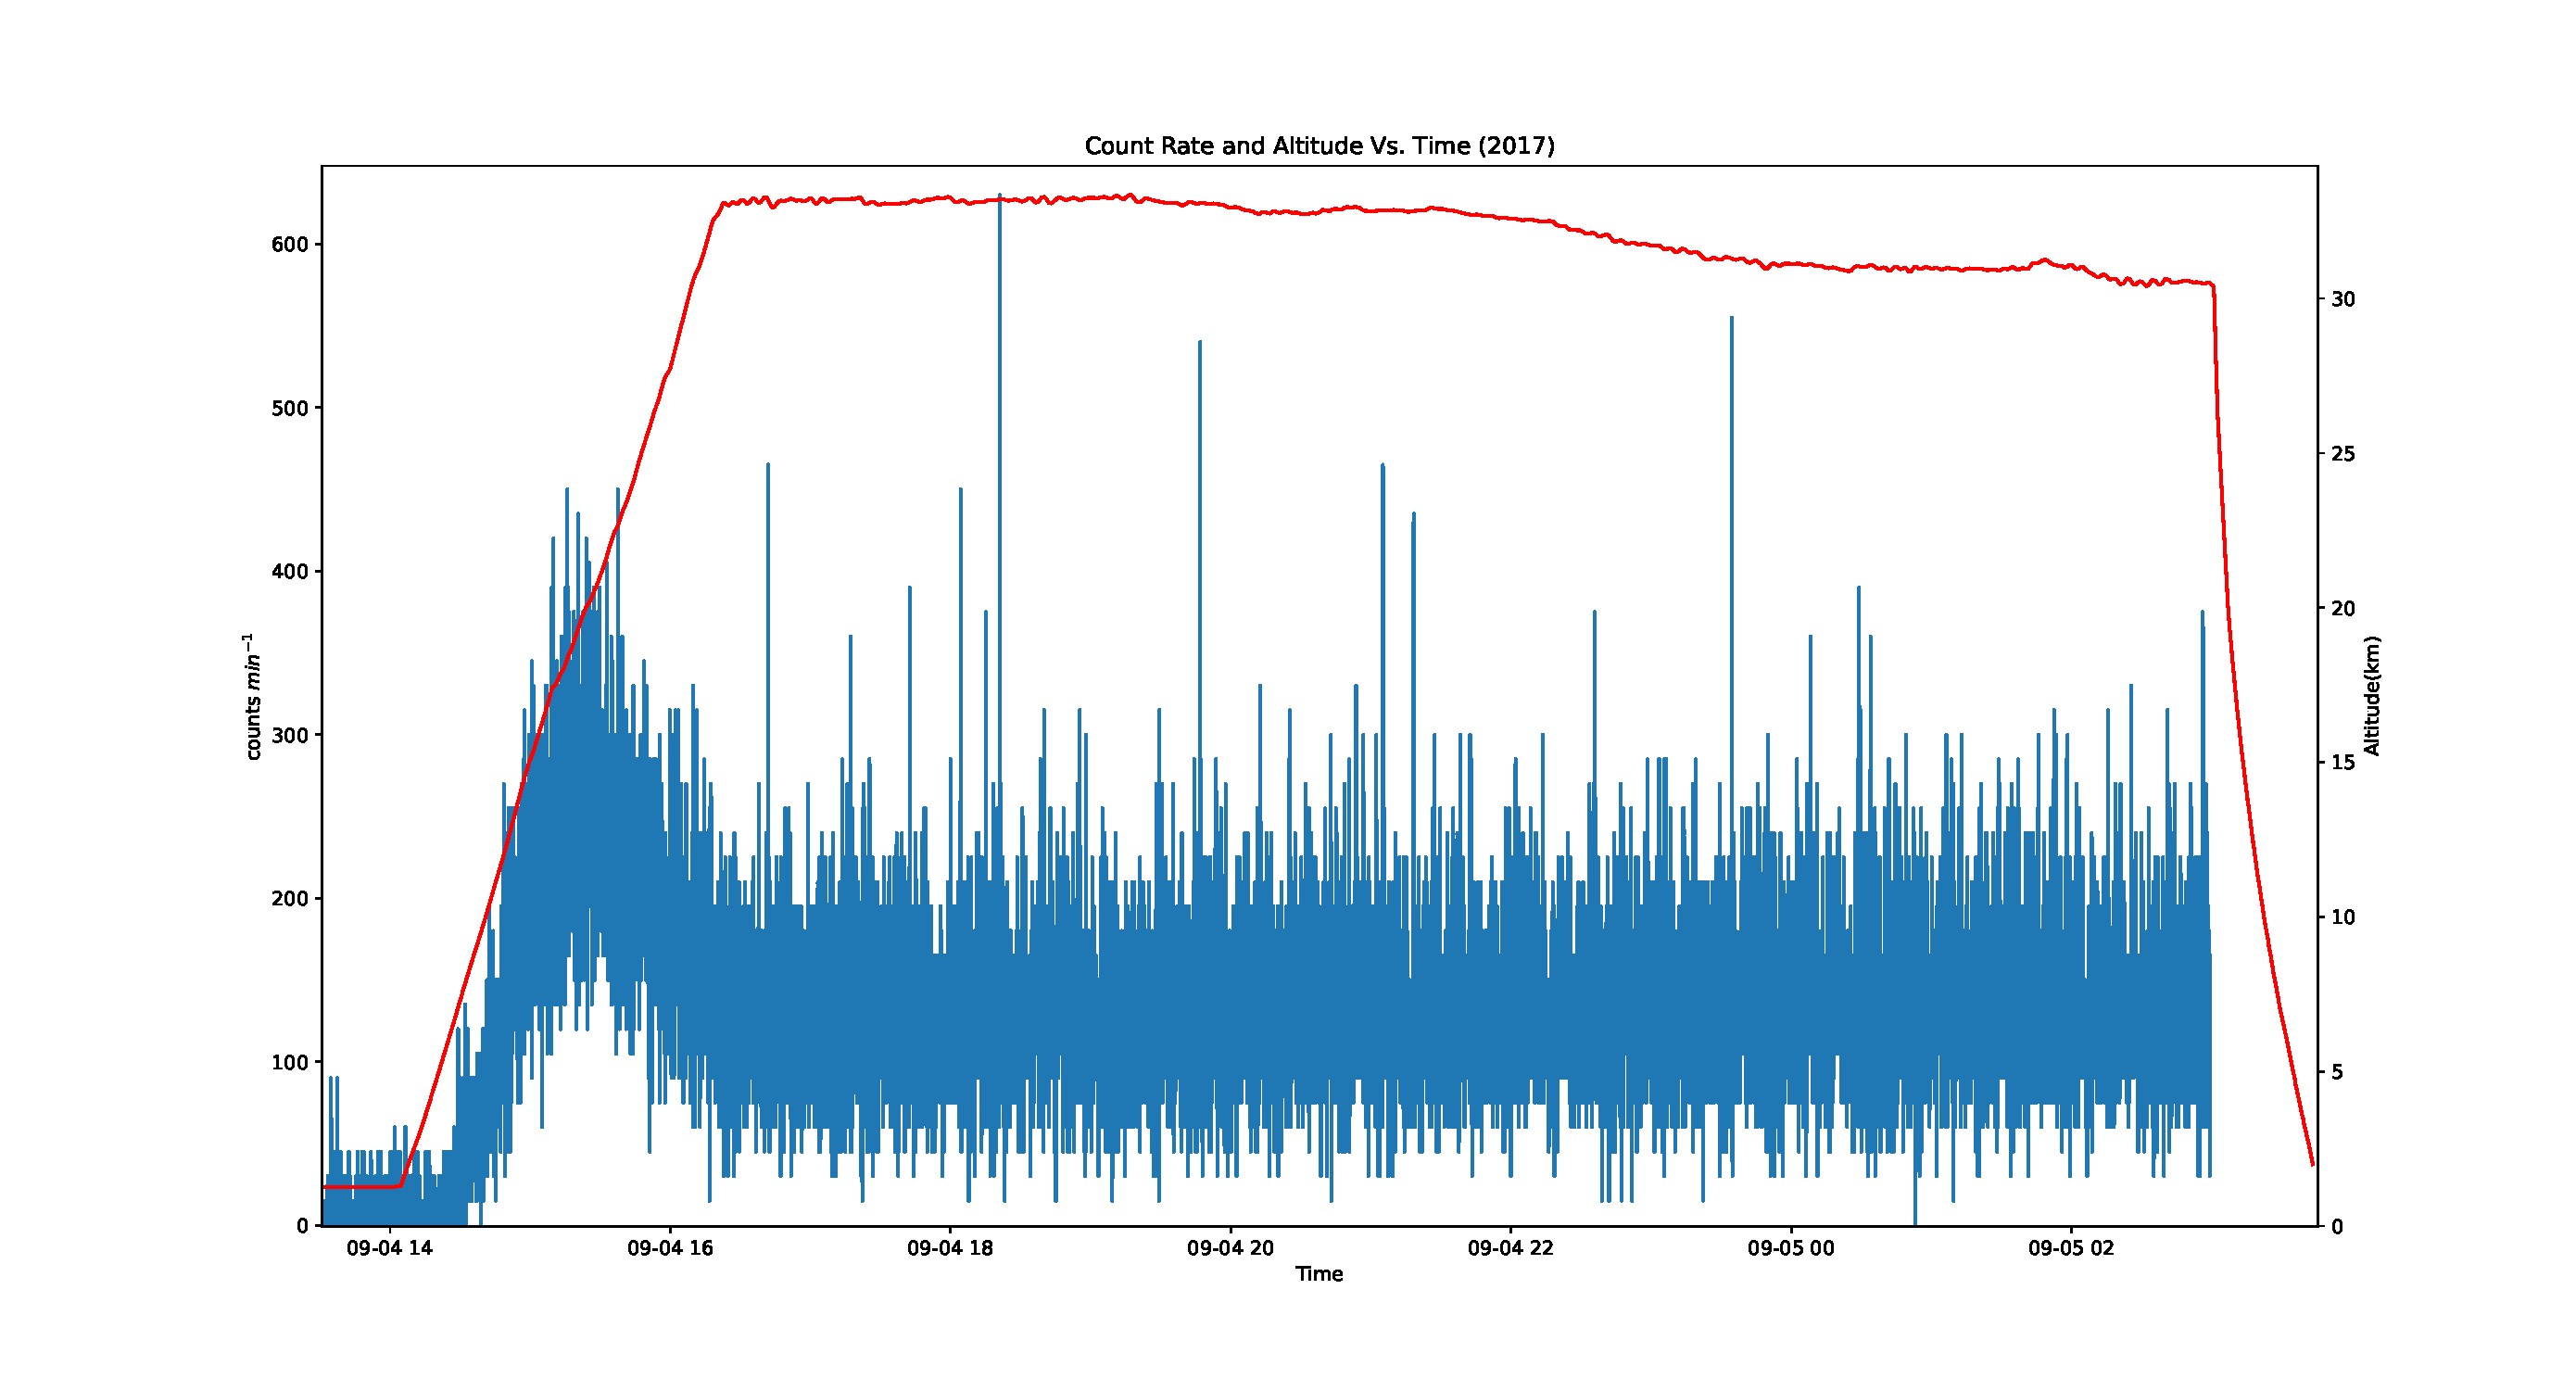
\includegraphics[width=\textwidth]{count_rate_altitude_2017.pdf}
\caption{Count Rate and Altitude vs Time for 2017 flight}
\label{fig:ratealttime_2017}
\end{figure}
%First:
%Present and characterize the first two plots - the data of the flight with counts vs altitude vs time.  Here we can talk about each flight and data shown.  Make sure to mention how the count rate changed as time and altitude changed.  We can talk about the flight time, the flight altitude variance, the coasting altitude, and how it all compares to the count rate.  We can be as descriptive as we can.
%mention the position of the pfotzer-regener maximum for both years.  Talk about discrepancies as the data shows.  Speculate in discussion later.

Both HASP balloons containing the SORA payloads were launched separately on September 4th on 2017 and 2018 respectively.  The MiniPIX was set to operate in Time over Threshold mode with a bias voltage of 4 Kev.  Frames were collected at static 4 second intervals during the 2017 flight and between 1 and 4 second intervals for the 2018 flight.  The complete flight altitude profiles with total count rates are shown in Figure~\ref{fig:ratealttime_2017} for 2017 and Figure~\ref{fig:ratealttime_2018} for 2018.

As shown in Figure~\ref{fig:ratealttime_2017} and Figure~\ref{fig:ratealttime_2018}, both flights have very similar flight profiles.  It took each flight about 2 hours and 30 minutes to ascend to a stable float altitude.  It is important to mention that the 2017 flight reach and maintained a float altitude of approximately $\SI{31.5}{\kilo\meter}$.  In contrast, the 2018 flight kept a float altitude of $\SI{37.2}{\kilo\meter}$.  The rate of decent was slow and steady for both flights.  As such, data was collected continuously throughout the whole flights.

With both flights reaching altitudes beyond $\SI{25.0}{\kilo\meter}$, the Pfotzer-Regener maximum was clearly observed.  In both Figure~\ref{fig:ratealttime_2017} and Figure~\ref{fig:ratealttime_2018}, the (WIP, please don't update me - Sam is working on this).

%Maybe compare to BEXUS flights and RADX flight as well, and mention how the maximum is similar - CONFIRM findings.


\begin{figure}[H]
\centering
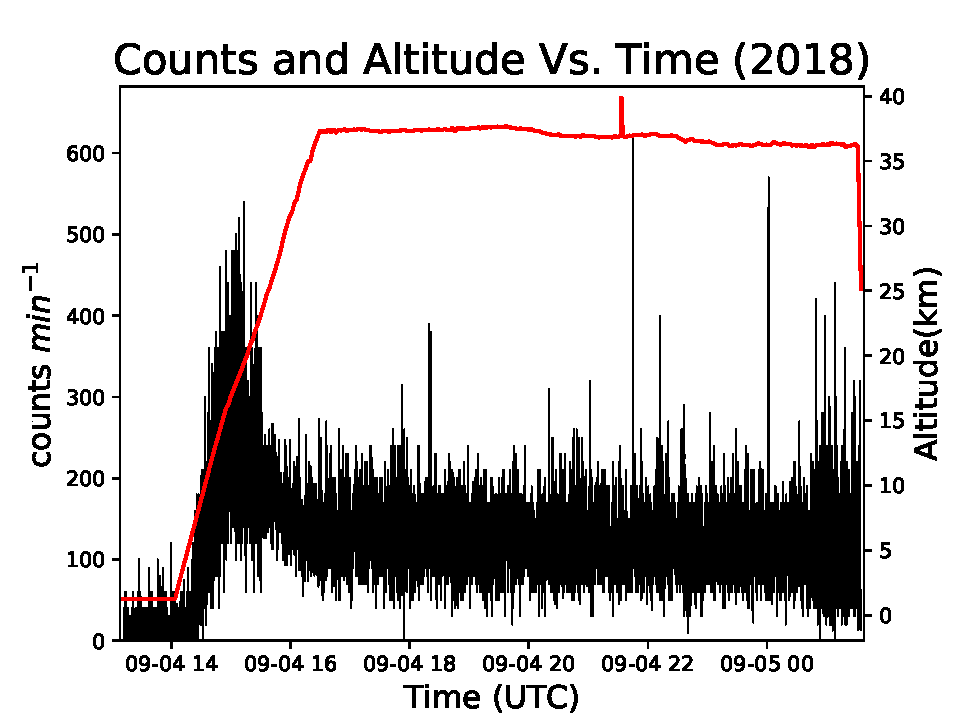
\includegraphics[width=\textwidth]{count_rate_altitude_2018.pdf}
\caption{PLACEHOLDER Count Rate and Altitude vs Time for 2018 flight}
\label{fig:ratealttime_2018}
\end{figure}

\begin{figure}[H]
\centering
\begin{subfigure}{.5\textwidth}
  \centering
  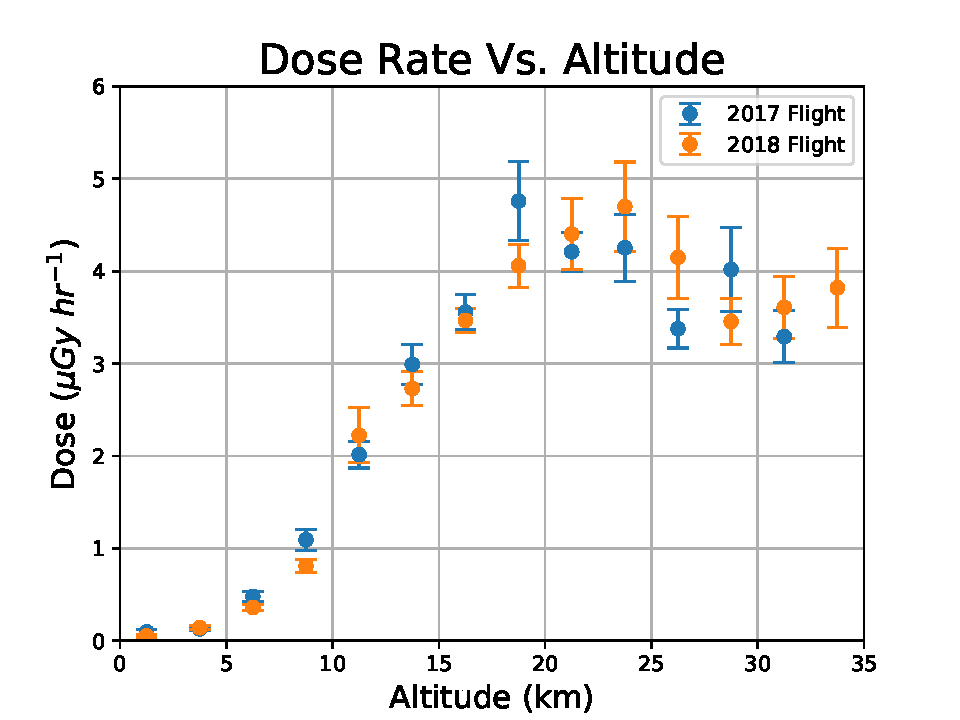
\includegraphics[scale=.45]{dva_stderr.pdf}
  \caption{Dose rate in silicon vs. altitude.}
  \label{fig:sub1}
\end{subfigure}%
\begin{subfigure}{.5\textwidth}
  \centering
  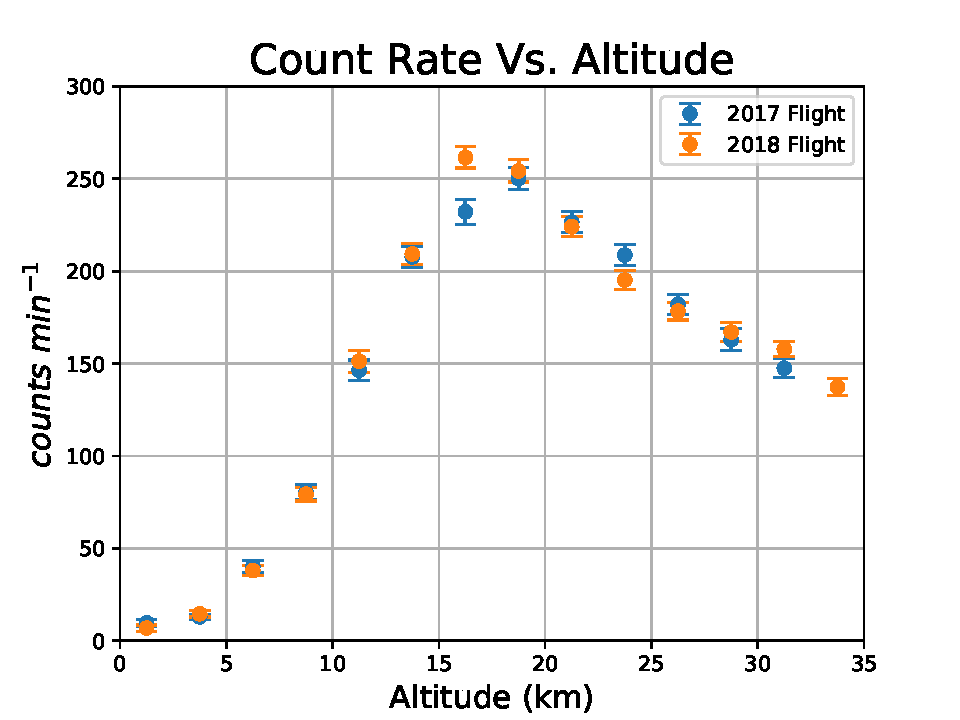
\includegraphics[scale=.45]{cva_stderr.pdf}
  \caption{Detector Hits vs. altitude.}
  \label{fig:sub2}
\end{subfigure}
\caption{Figure ~\ref{fig:sub1} shows the absorbed dose rate per hour as a function of altitude from the MiniPIX.  Figure ~\ref{fig:sub2} shows the counts per minute as a function of altitude again from the MiniPIX data.}
\label{fig:test}
\end{figure}
%Next, go into the absorbed rate vs altitude plot.  Mention how the LET varies for materials such as silicon and muscle.  Go into the pfotzer-regener maximum again, compare.  Compare this to the accompanying figure, Detector Hits vs Altitude.  There is a slight discrepancy in the flights, this may be useful to mention.  All error bars are 1 sigma standard deviation.

\begin{figure}[H]
\centering
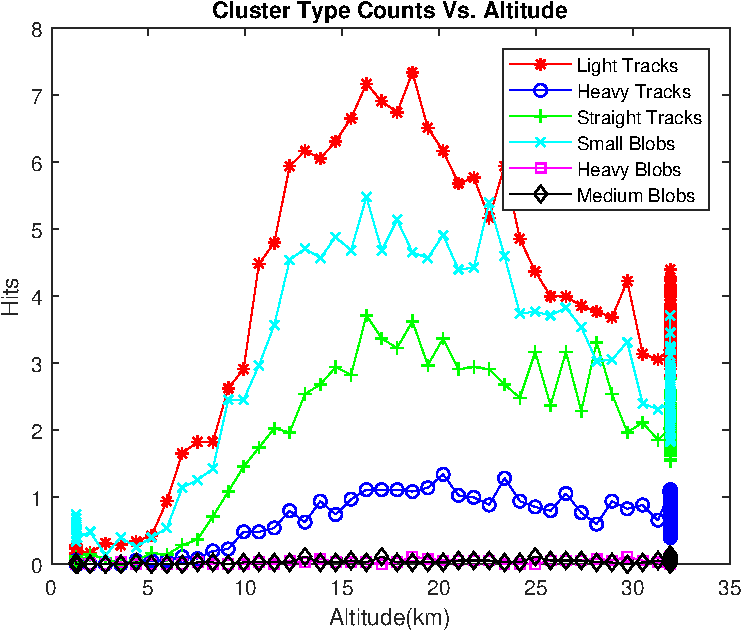
\includegraphics[scale=.75]{ctva-cropped.pdf}
\caption{Cluster Type Counts vs. altitude.}
\end{figure}
%Finally, the last figure Cluster Type Counts vs Altitude.  This is useful due to the MiniPIX being able to analyze indivudual track lenghts.  From here, these tracks can be characterized into different and indidivual categories.  This is useful for LET calculations and overall more precise for dosage calculations.  It may also help with particle identification.  Notice how the heavier tracks and medium blobs are all in the low counts yet they still vary somewhat with altitude (hard to see).

\begin{figure}[H]
\centering
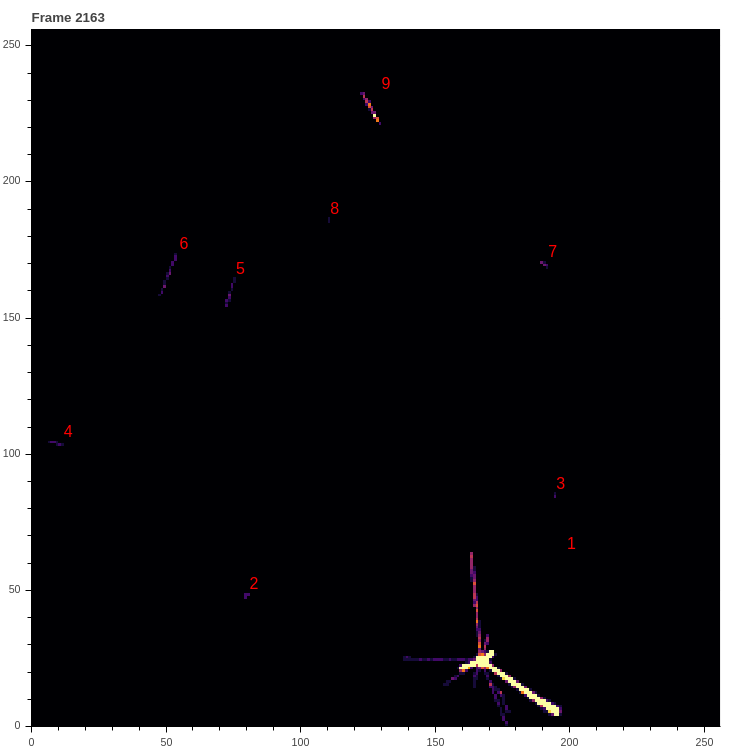
\includegraphics[scale=.35]{tracks.png}
\caption{Frame collected at float.}
\end{figure}

